% !TeX root = ..\..\main.tex
\section{Data Integrity}

We begin by first running a summary on the data to ensure that all the values are within the ranges we would expect.

\lstinputlisting[caption={Summary of Data}]{Sections/DataIntegretity/Outputs/summary.txt}

We can see that our data ranges are appropriate for our date and time columns however, without prior knowledge of the range of overturning strength it is difficult to detect outliers. We may attempt to do so using a box plot

\begin{figure}[H]
    \centering
    \begin{subfigure}[b]{\sOneSize\textwidth}
        \centering
        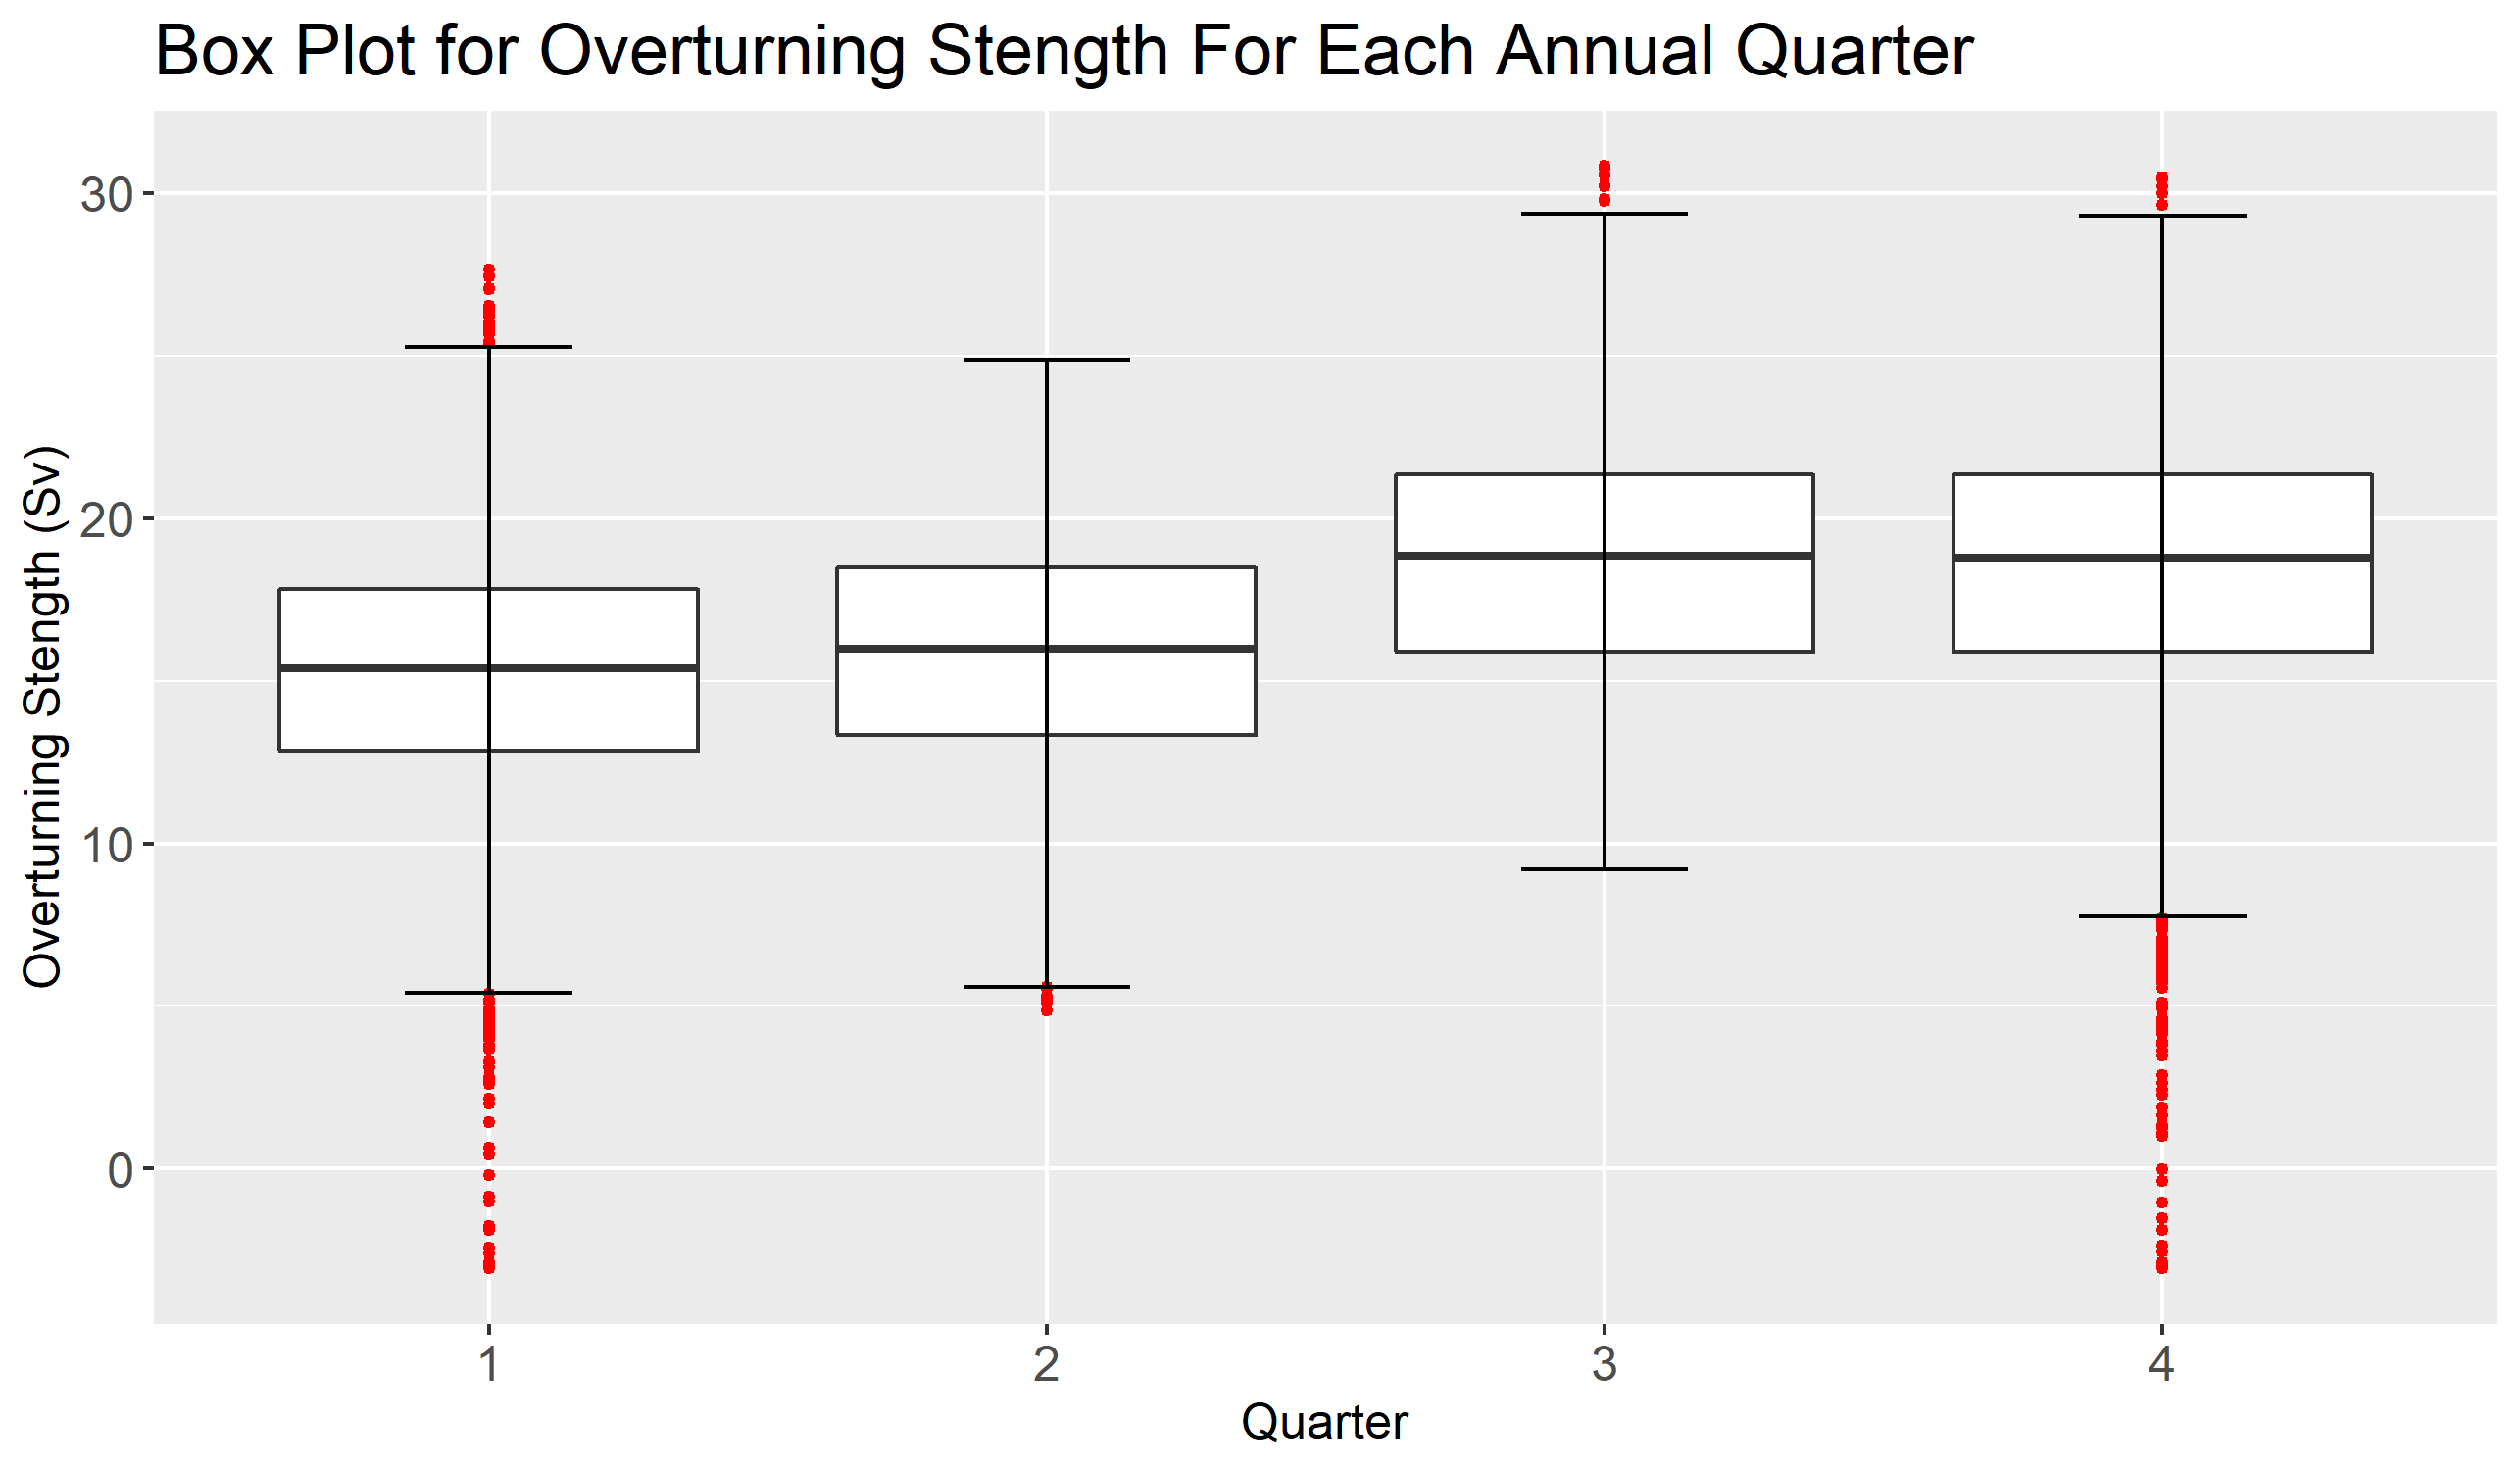
\includegraphics[width=\textwidth]{Sections/DataIntegretity/Plots/Box(yr).png}
        \subcaption{Data grouped into annual quarters.}
    \end{subfigure}
    \begin{subfigure}[b]{\sOneSize\textwidth}
        \centering
        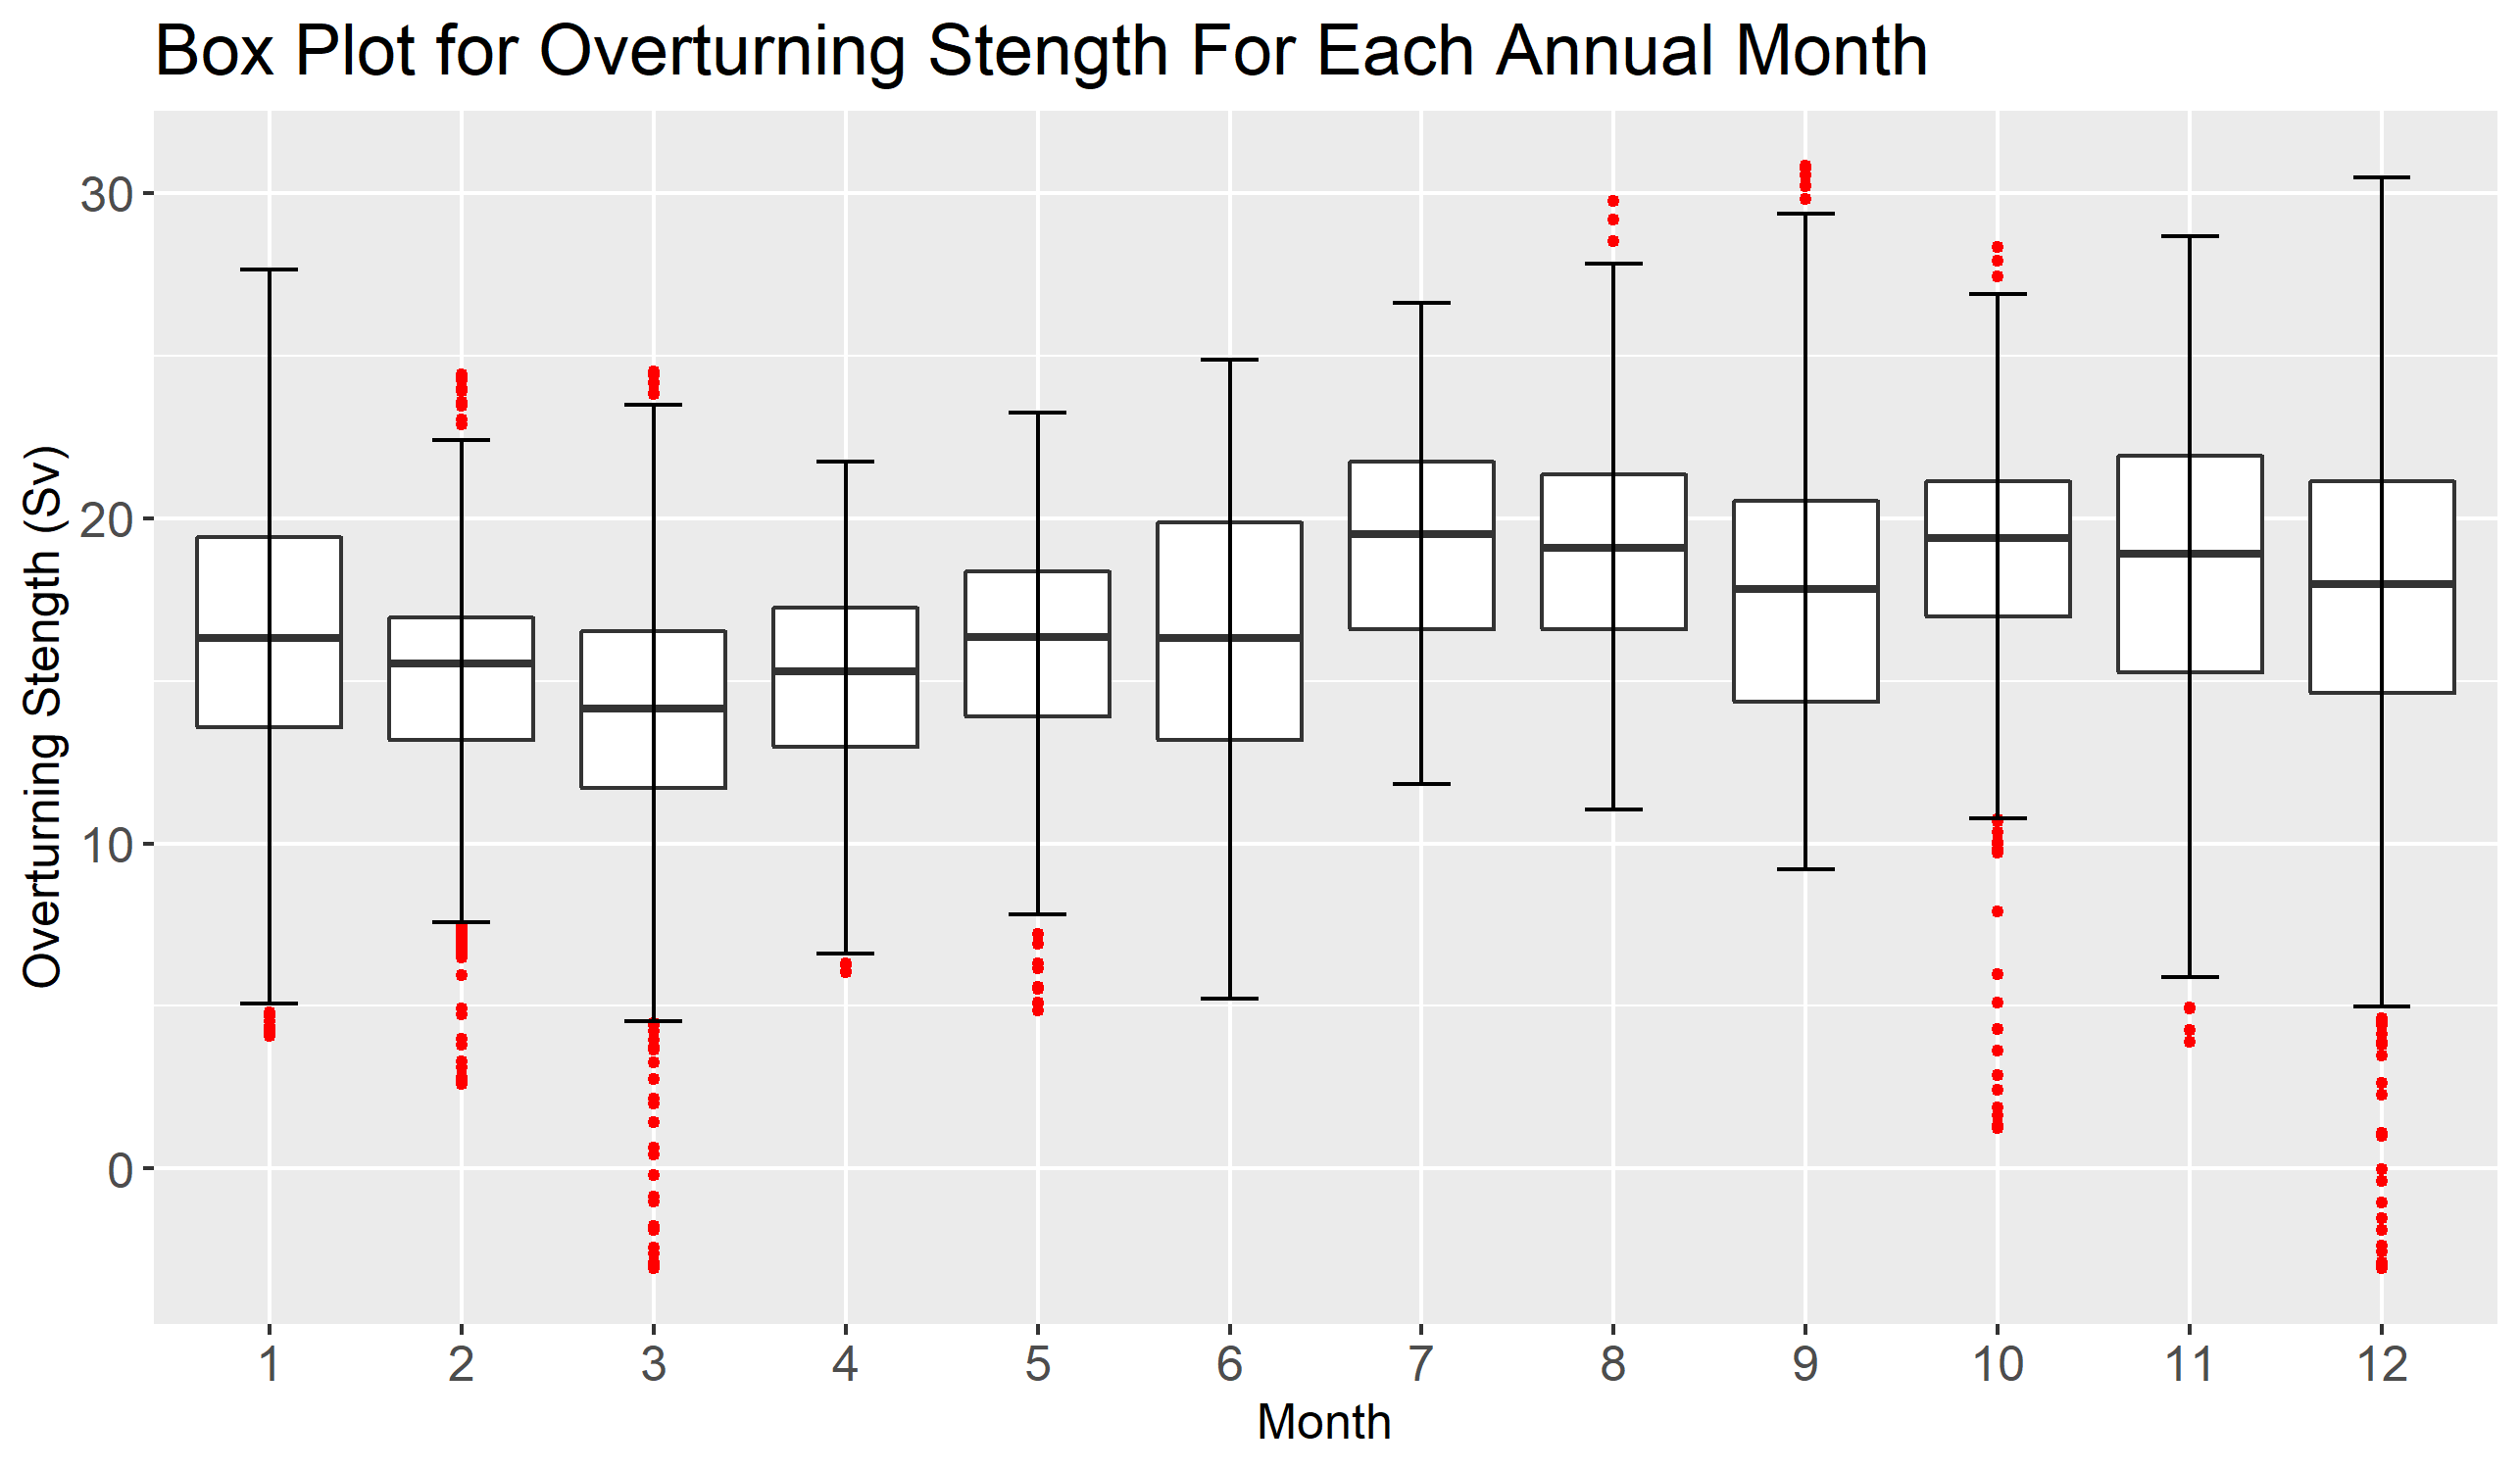
\includegraphics[width=\textwidth]{Sections/DataIntegretity/Plots/Box(mnth).png}
        \subcaption{Data grouped into annual months.}
    \end{subfigure}
\caption{Box plot showing the distribution of overturning strength (Sv) for both annual quarters and for each month. Outliers defined as $\frac{3}{2}\IQR$ from the upper or lower quartiles are highlighted in red.}\label{S1fig:boxplot(yr)}
\end{figure}
We can see in \autoref{S1fig:boxplot(yr)} which uses the interquartile range as a method to detect outliers we find an extremely high number of outliers especially in the first and fourth quartile. To investigate further into these outliers we can extract them from our data and plot them against time.
\nline
Looking at \autoref{S1fig:outliers.ts} we can see that the outliers tend to be grouped together but are spread well throughout the data. We may then conclude that these outliers are instead byproducts of the complex nature and long term trends of the ocean.

\begin{figure}[H]
    \centering
    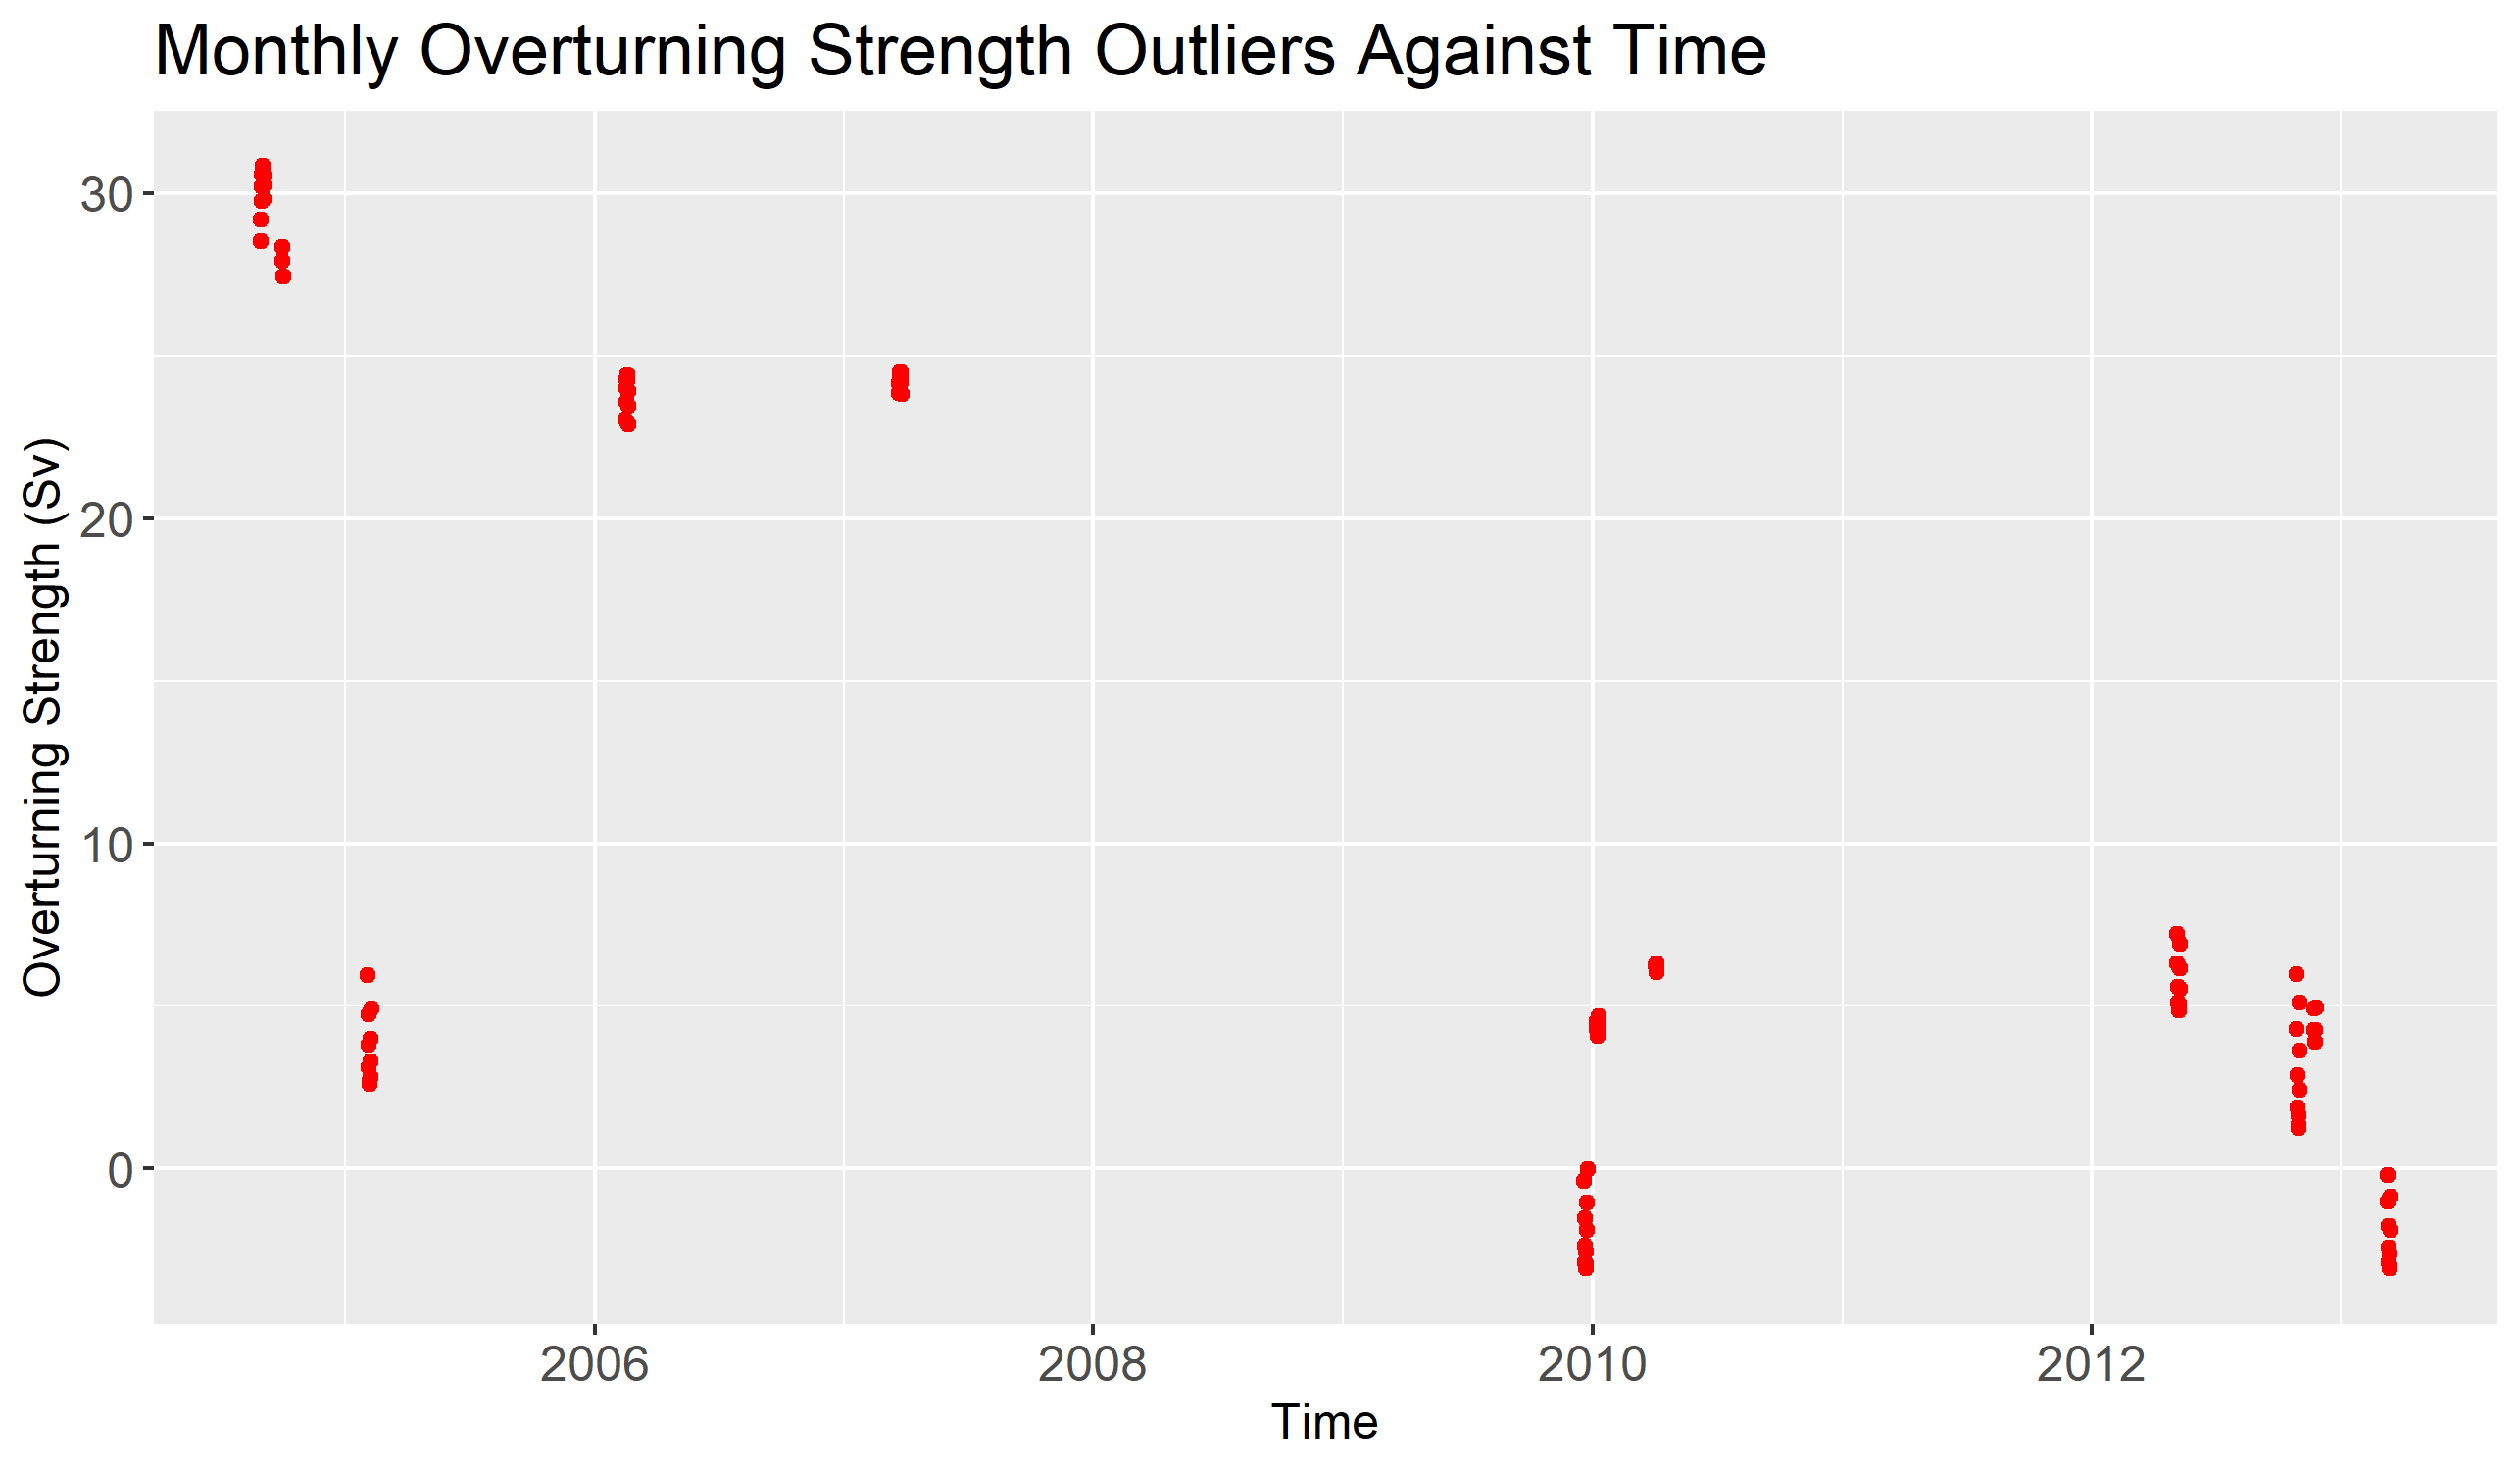
\includegraphics[width=\sOneSize\textwidth]{Sections/DataIntegretity/Plots/outliers.png}
    \caption{Monthly overturning strength outliers plotted against time.}
    \label{S1fig:outliers.ts}
\end{figure}

To get an overview of our data we begin by grouping it into years and annual quarters and then take the mean of each group. This is to reduce noise in our data and also reduces the number of points which helps speeds up the model building computation. We can see this data as a time series in \autoref{S2fig:orig.ts}.

\begin{figure}[H]
    \centering
    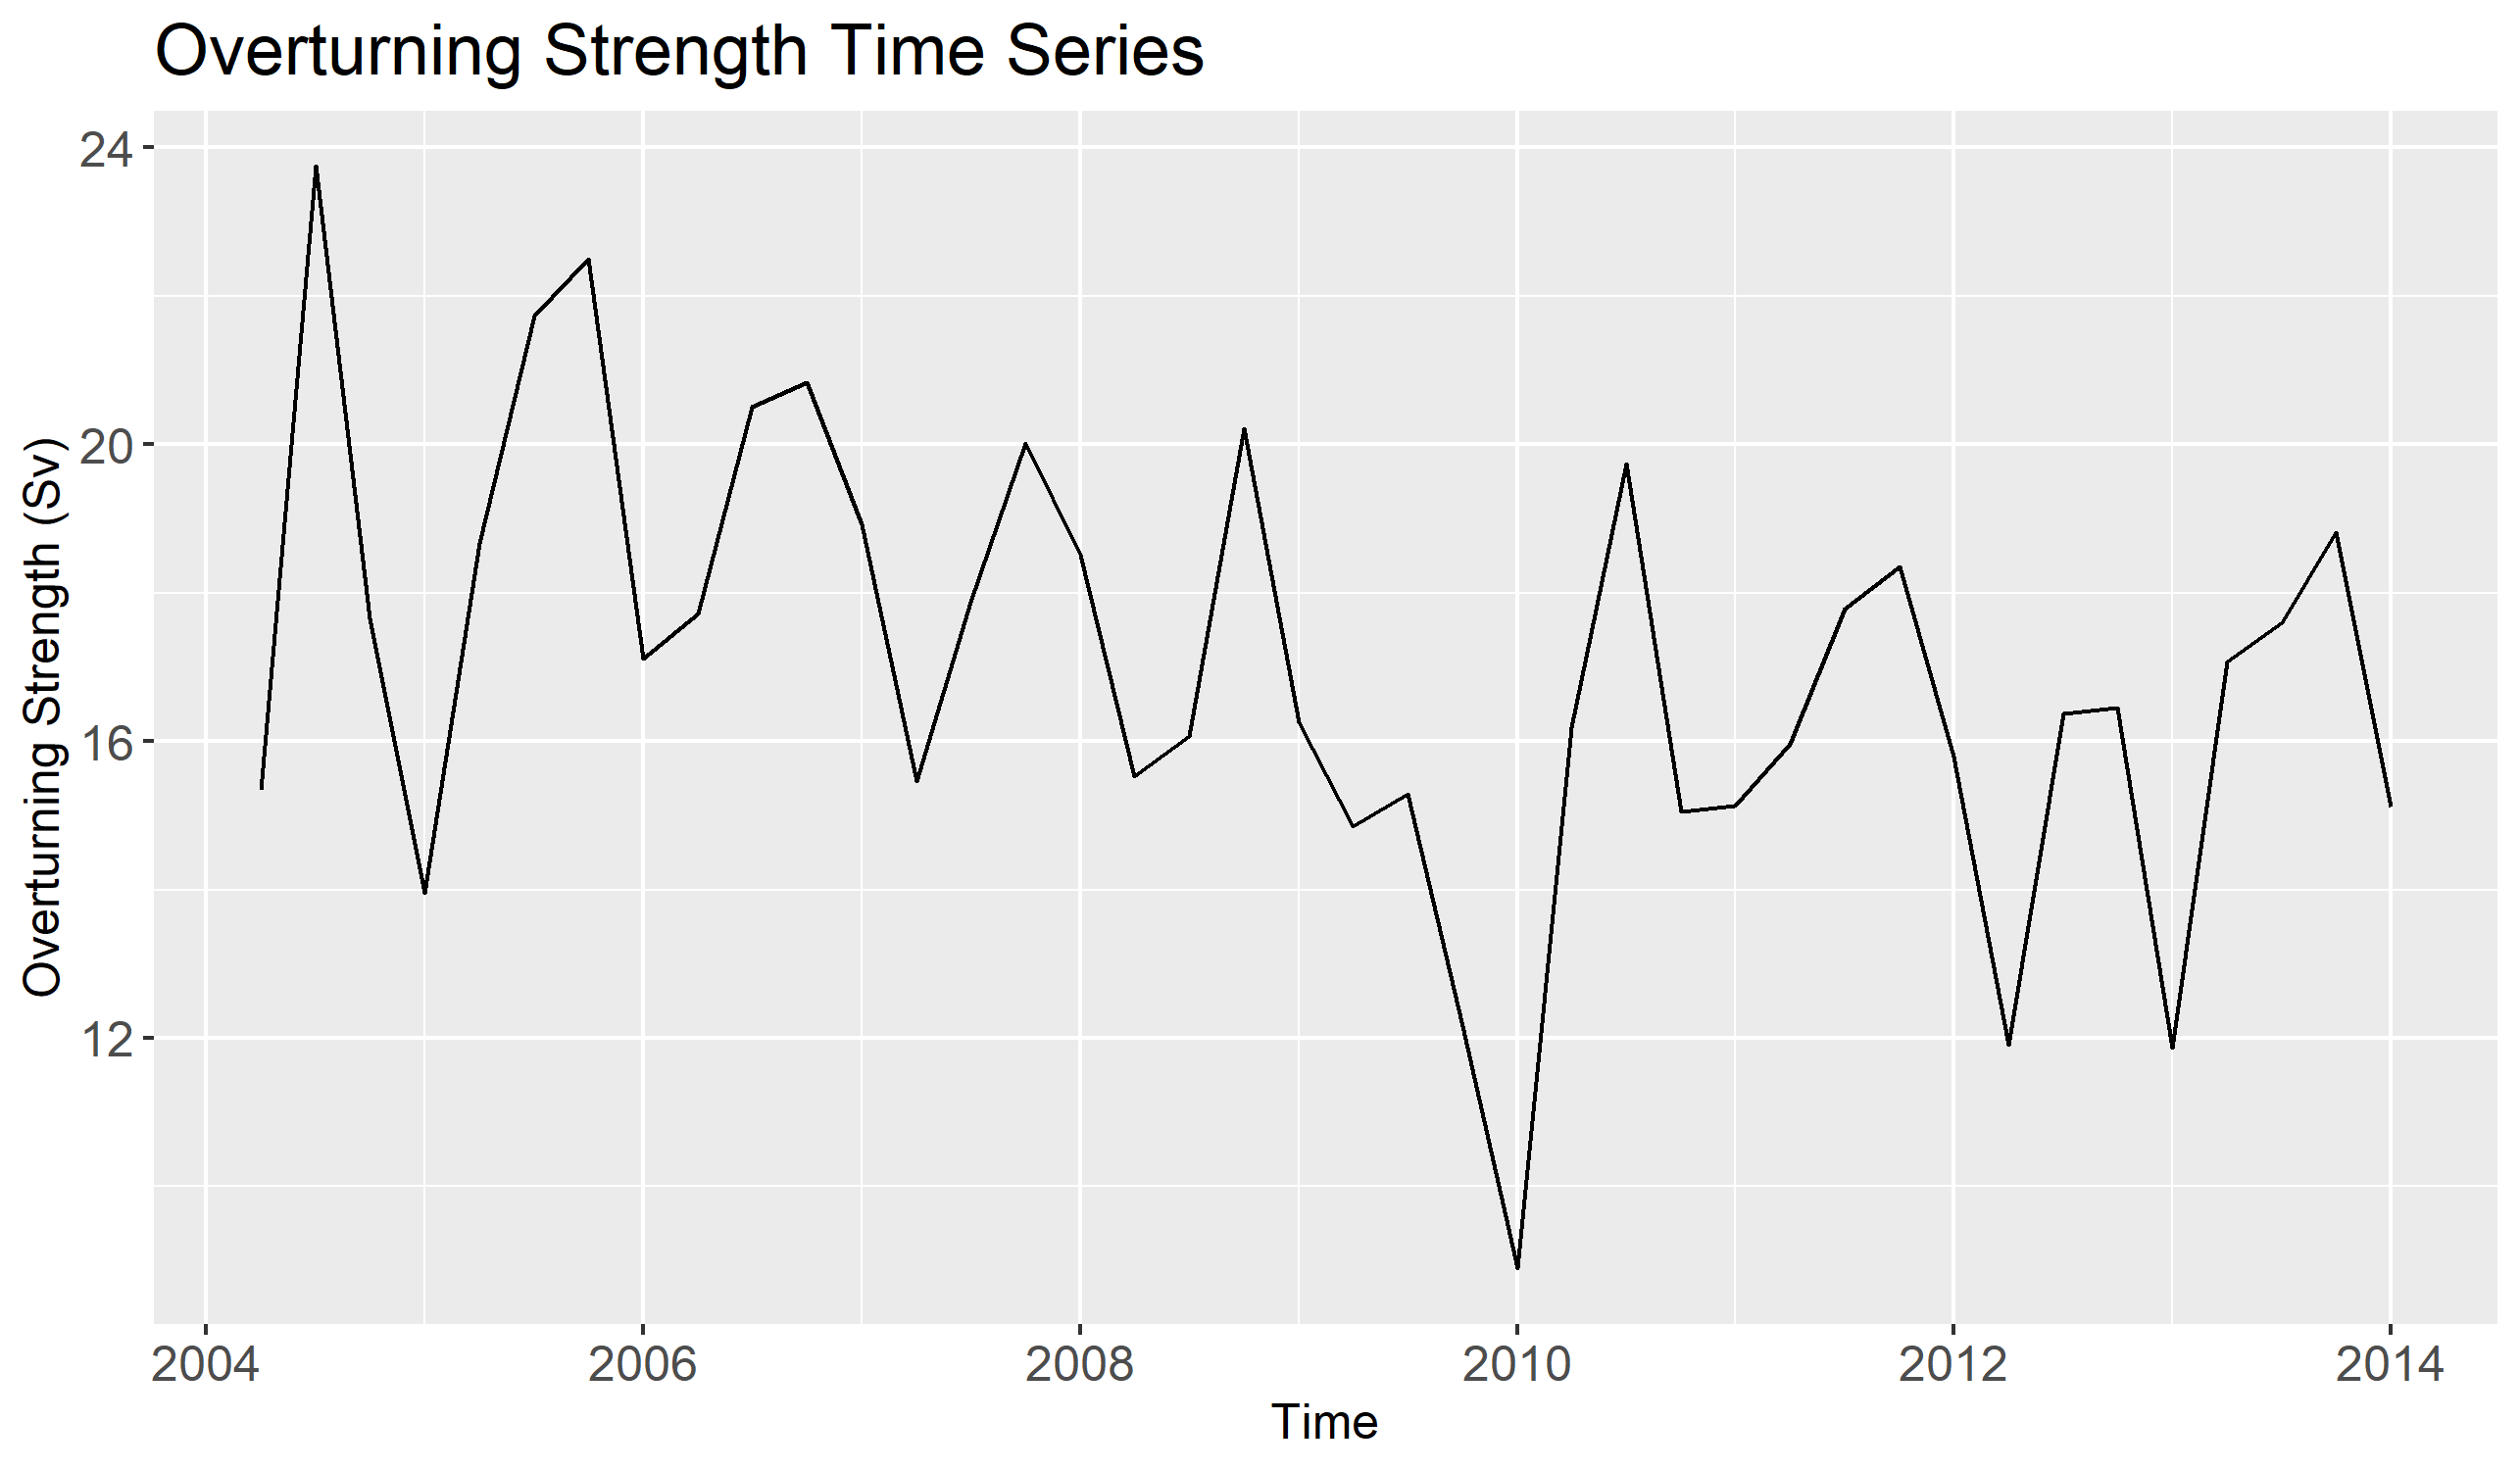
\includegraphics[width=\sOneSize\textwidth]{Sections/DataIntegretity/Plots/orig.png}
    \caption{A time series of our original data where each point is the mean taken over the annual quarter.}
    \label{S2fig:orig.ts}
\end{figure}

Taking a look at \autoref{S2fig:orig.ts} we can see that there appears to be a pattern of changing between up and down within fairly consistent values roughly every half of year. However, this pattern is not followed between 2009 and 2011 when we see a drop shortly followed by another drop before a very sharp upwards tick till halfway through 2010. Whilst this significant drop may seem as an outlier it is generally accepted in the literature, and its origin is uncertain \cite{reduction.cite}.
\nline
With this quick assessment of the data concluding that there are no outliers, we will then continue to build our models without removing any data from the provided data set.